\section{Forecast Evaluation and Confidence Analysis}

This section presents a detailed evaluation of the future observations forecasts for each of the statistical time series models developed: the Automatic SARIMA model, the Manual SARIMA model, the STL Decomposition followed by ARIMA Modeling (STLM), and the Exponential Smoothing State Space Model (ETS). For each model, we analyze the visual representation of the forecast against actual data, interpret the associated confidence intervals, and the accuracy values.

\subsection{Automatic SARIMA Model}

The SARIMA(2,0,0)(0,1,2)[12] model, automatically selected, was utilized to forecast the next 41 observations, covering the entire test set period. \\

\begin{figure}[H]
    \centering
    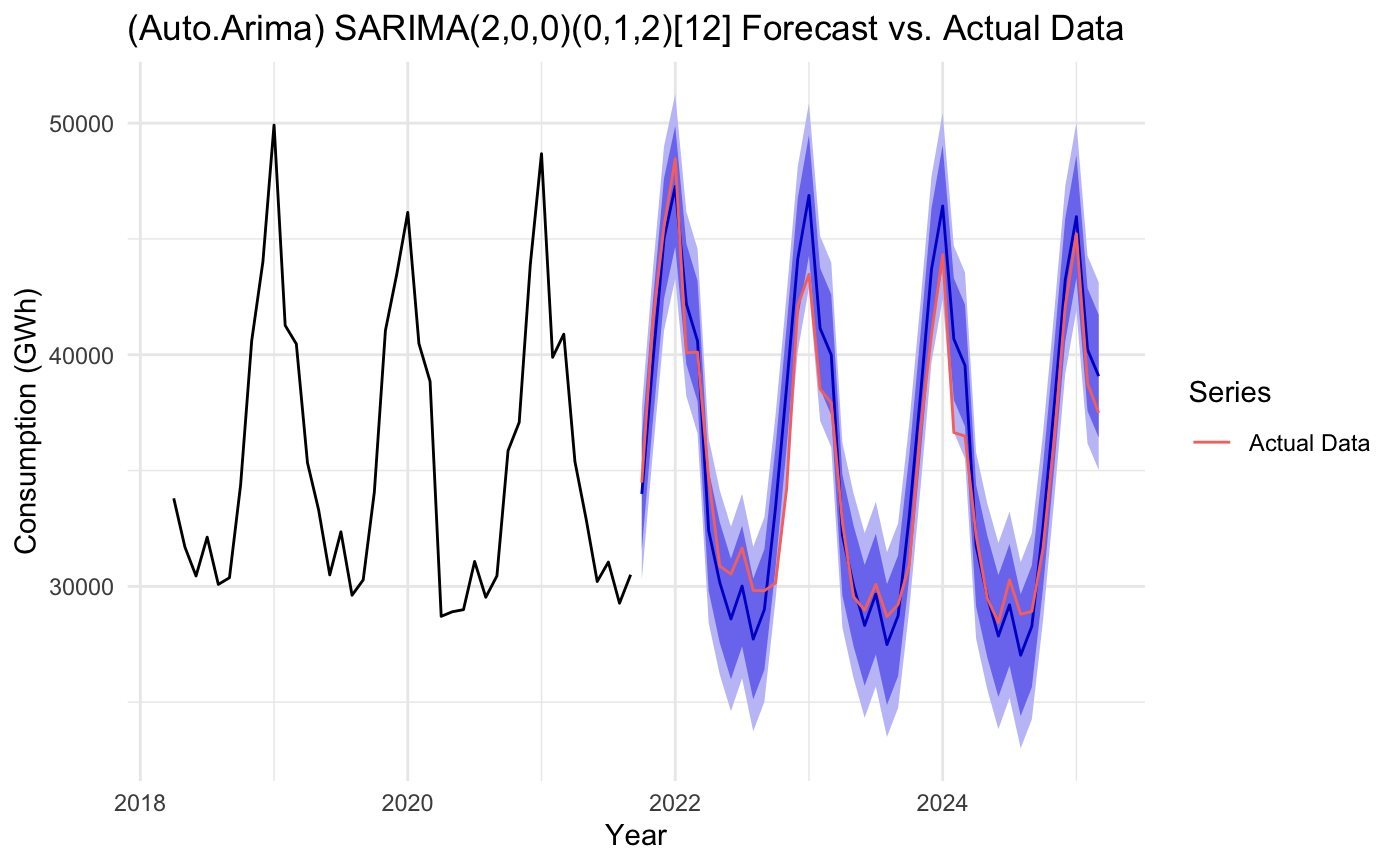
\includegraphics[width=1\linewidth]{images/for_auto.png}
    \caption{(Auto.Arima) SARIMA(2,0,0)(0,1,2)[12] Forecast vs. Actual Data}
    \label{fig:enter-label}
\end{figure}

The forecast plot for the Automatic SARIMA model shows strong performance over time. The forecast is accompanied by blue-shaded bands representing uncertainty levels: a darker band indicates higher confidence (95\%), while a lighter band denotes lower confidence (80\%). Crucially, most of the observed values (represented by the red line) fall within the 95\% confidence intervals. This indicates that the model is highly effective at capturing both the underlying trend and the variability of the electricity consumption series. Furthermore, the model accurately reproduces the regular seasonal patterns, with the confidence intervals successfully encompassing the extremes of the historical data, demonstrating a good fit to the seasonality. The gradual widening of these bands over time is an expected characteristic of time series forecasting, reflecting the increasing uncertainty in longer-term predictions.\\

Regarding forecast accuracy, the Mean Absolute Percentage Error (MAPE) on the test set was 4.37\%. This signifies that, on average, the model's forecasts deviated from the actual values by approximately 4.5\%. This is considered a high level of accuracy. The Root Mean Squared Error (RMSE) provides a measure of the typical error magnitude in Gigawatt-hours (GWh). The Theil's U statistic for the test set was 0.518, which is less than 1, confirming that this model outperforms a simple naive forecasting approach. While improved from the training set, the autocorrelation function at lag 1 (ACF1) of 0.619 on the test set suggests that some residual autocorrelation remains, implying that there might still be uncaptured patterns in the error term.\\

\subsection{Manual SARIMA Model}

The manually configured SARIMA(1,1,1)(0,1,1)[12] model was also used to generate forecasts, which were subsequently evaluated against the actual values within the test set.\\

\begin{figure}[H]
    \centering
    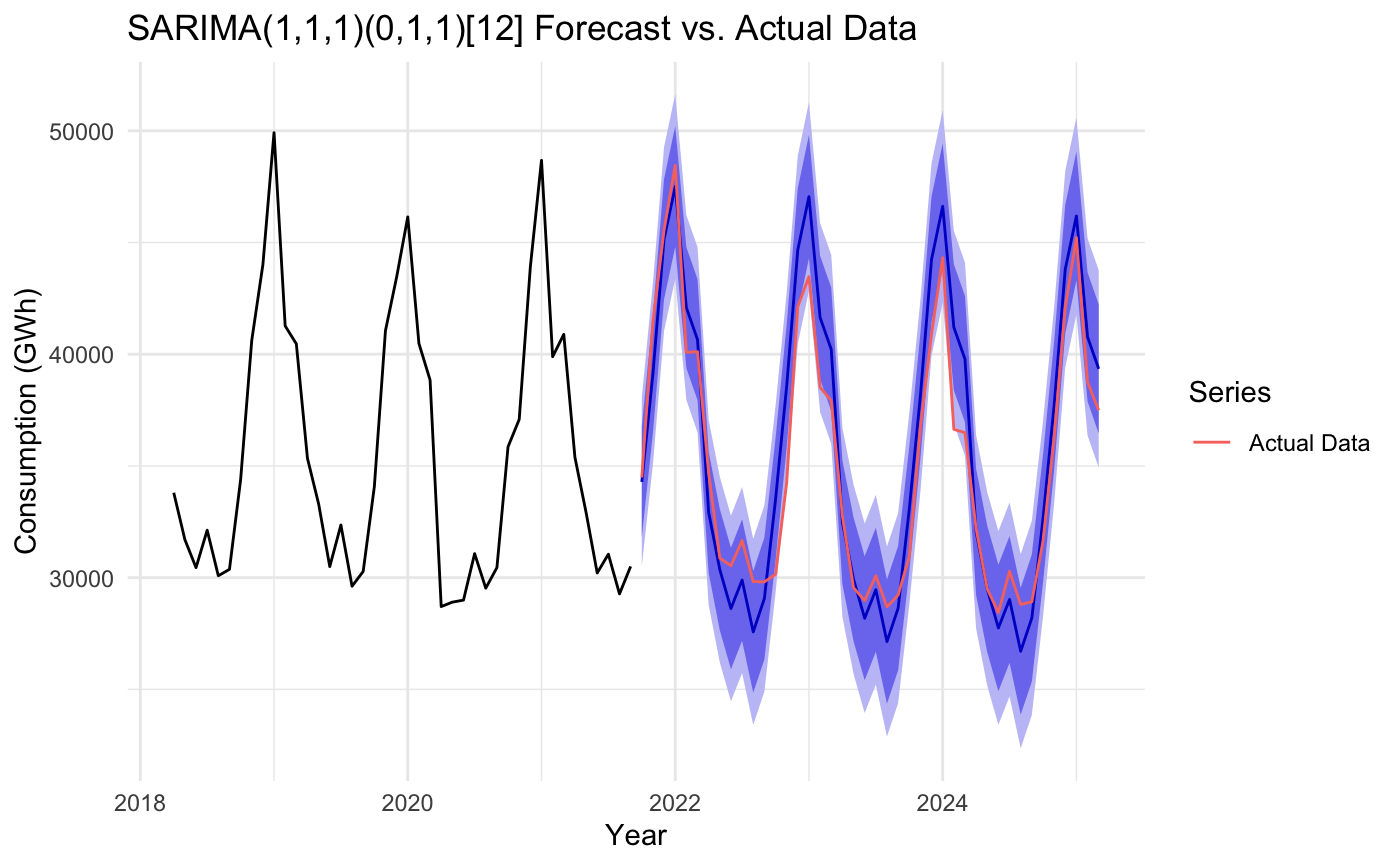
\includegraphics[width=1\linewidth]{images/for_ma.png}
    \caption{SARIMA(1,1,1)(0,1,1)[12] Forecast vs. Actual Data}
    \label{fig:enter-label}
\end{figure}

Similar to the automatically selected SARIMA model, the manually configured SARIMA forecast also exhibited good performance when compared to the actual data. The confidence bands, represented by blue shading, follow the same interpretation as before: darker shades indicate higher confidence (95\%), and lighter shades indicate lower confidence (80\%). The majority of the actual values (red line) remained within the 95\% confidence intervals, suggesting that the model effectively captured the trend and variability of the series throughout the forecast period. The seasonal patterns observed in the actual data were well replicated by the model, further indicating a good fit to the series' seasonality. The widening of the confidence bands over time is a typical and expected behavior in time series models, reflecting increasing uncertainty as the forecast horizon extends.\\

In terms of forecast accuracy, the Mean Absolute Percentage Error (MAPE) on the test set was 4.67\%. This remains a very good value, demonstrating a high level of accuracy. The Theil's U statistic of 0.558 (below 1) validates the model's predictive utility by confirming its outperformance of a naive prediction. While absolute and percentage errors naturally increased on the test set compared to the training set, they remained at acceptable levels. However, a notable increase in the autocorrelation of the residuals (ACF1 = 0.657) was observed on the test set. This suggests that the model might not have fully captured all underlying patterns in the future data, implying that exploring other SARIMA orders could potentially lead to further improvements.\\

\subsection{STL Decomposition Followed by ARIMA Modeling}

The STL + ARIMA(2,1,1) model, which first decomposes the time series and then applies ARIMA to the remainder, was assessed for its future forecasts.\\

\begin{figure}[H]
    \centering
    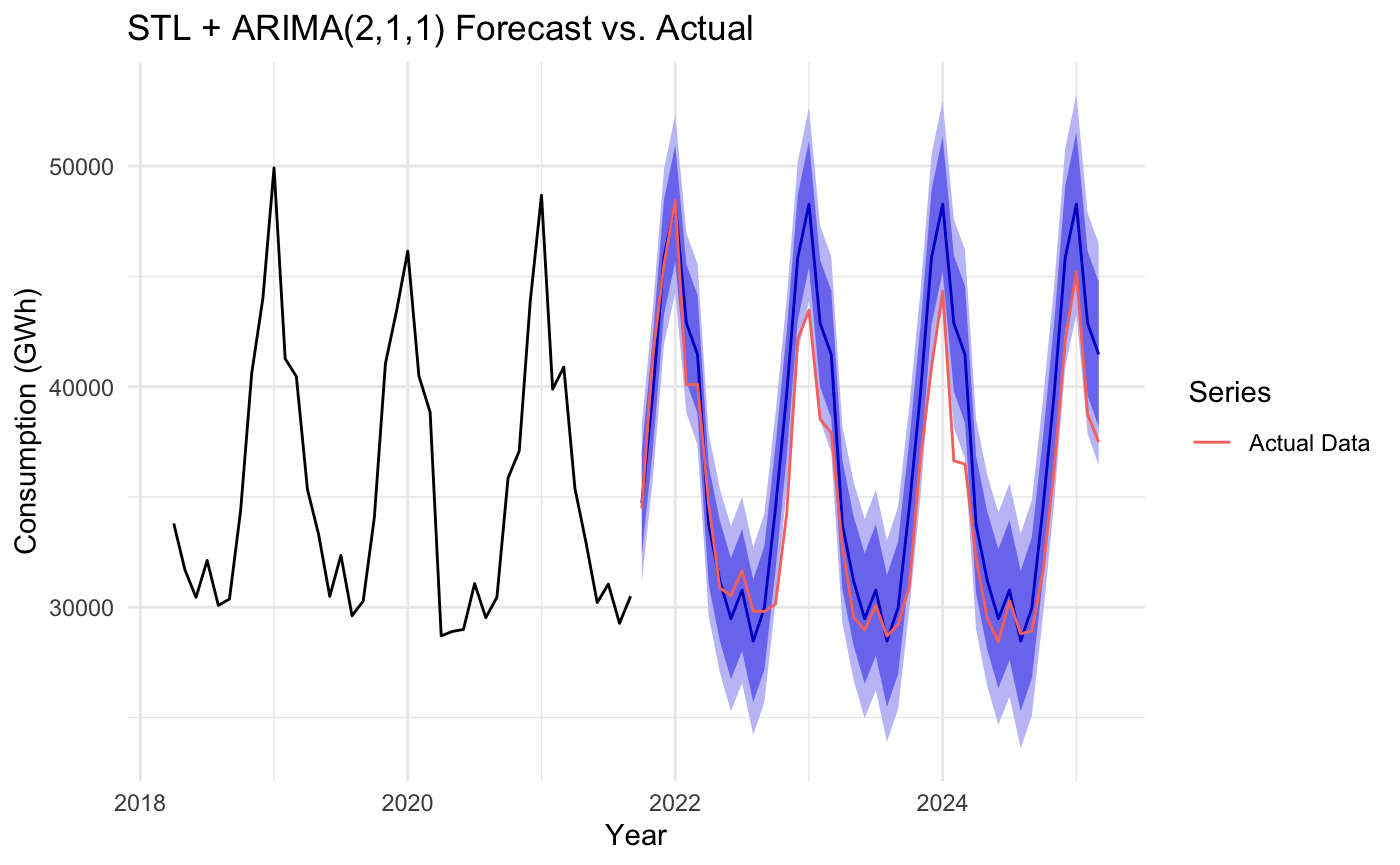
\includegraphics[width=1\linewidth]{images/for_stml.png}
    \caption{STL + ARIMA(2,1,1) Forecast vs. Actual}
    \label{fig:enter-label}
\end{figure}

The forecast generated by the STL + ARIMA(2,1,1) model showed satisfactory results over time. The confidence bands, indicating uncertainty, were present and interpreted similarly to the SARIMA models. While the actual values (red line) largely remained within the 95\% confidence intervals, unlike the SARIMA models, there were instances where they only fell within the 80\% range or even outside the intervals. Nevertheless, the model generally managed to capture the trend and variability of the time series well for most of the forecast horizon. The seasonal patterns inherent in the data were adequately represented, reflecting the effectiveness of the seasonal decomposition performed by the STL method. The expected widening of the confidence bands over time confirmed the natural increase in uncertainty for more distant forecast periods.\\

For forecast accuracy, the model exhibited good training performance, with training residuals closely resembling white noise (ACF1 $\approx$ 0) and a MASE (Mean Absolute Scaled Error) less than 1, along with a MAPE of approximately 3\%. This indicates strong in-sample performance. However, a significant deterioration in performance was observed on the test set, with all error metrics increasing substantially ($MAPE > 6\% $ and  $MASE > 1$). The high ACF1 of 0.69 on the test set points to strong autocorrelation in the errors, suggesting underfitting to the most recent data. This indicates that the model might not have captured new patterns or recent structural changes specific to the test period, or that the chosen ARIMA order for the residuals was inappropriate, leading to out-of-sample underfitting. The Theil's U value of 0.779 suggests it still performs better than a naive forecast, but less effectively than the SARIMA models.\\

\subsection{Exponential Smoothing State Space Model (ETS)}

The ETS model was employed to generate forecasts for future electricity consumption.\\

\begin{figure}[H]
    \centering
    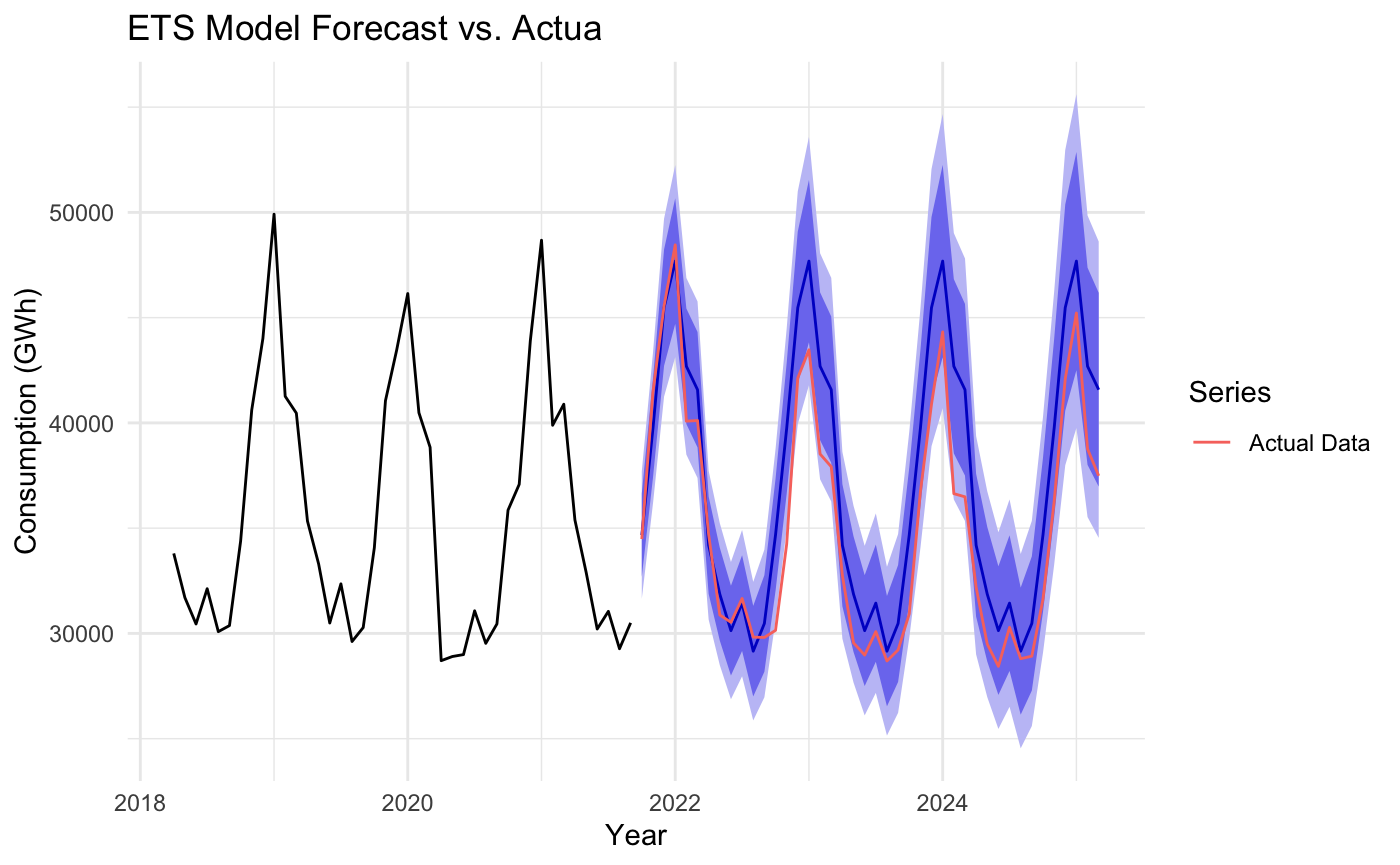
\includegraphics[width=1\linewidth]{images/for_ets.png}
    \caption{ETS Model Forecast vs. Actual}
    \label{fig:enter-label}
\end{figure}

Similar to the SARIMA models, the ETS forecast also showed good results over time. The blue-shaded bands represented the familiar uncertainty levels (95\% and 80\% confidence). Most of the observed values (red line) stayed within the 95\% confidence intervals, indicating that the model effectively captured both the trend and variability of the series. The regular seasonal patterns were well-represented, with the intervals successfully capturing the extremes of the historical series, suggesting a good fit to the seasonality. The widening of the confidence bands over time, reflecting increasing uncertainty for longer-term forecasts, was also an expected behavior.\\

In terms of forecast accuracy, on the training set, the model fit well with relatively low error rates (MAPE $\approx$ 3.2\%) and better performance than the naive model ($MASE < 1)$. However, on the test set, errors increased significantly ($MAPE > 6\%$, $MASE > 1$), pointing to poorer out-of-sample performance. Additionally, the high residual autocorrelation on the test set (ACF1 $\approx$ 0.65) suggests that the model did not fully capture all the series' patterns, possibly due to underfitting or shifts in the data's underlying dynamics. The Theil's U value of 0.787 confirms that the ETS model performs better than a naive forecast, but its performance on the test set is notably weaker compared to both SARIMA models.\\


